\documentclass[a4paper]{jpconf}
\usepackage{graphicx}
\usepackage[margin=0.8in]{geometry}
\usepackage{lmodern}% http://ctan.org/pkg/lm
\usepackage{listings}
\usepackage[utf8]{inputenc}
\usepackage{wrapfig}
\usepackage{listings}
\usepackage{citesort}
\usepackage{changepage}
\usepackage{caption}
\usepackage{color}
\usepackage{subcaption}
\usepackage{hyperref}\begin{document}
\title{Profiling ATLAS Kit Validation on \newline Intel Haswell-EP processors}

\author{M Guerri$^1$, D Giordano$^1$, C Cordeiro$^1$}
\address{$^1$ CERN}
\ead{marco.guerri@cern.ch}

\definecolor{lightblue}{gray}{0.95}

\lstset{
    language=Python,
    basicstyle=\fontfamily{pcr}\small,
    tabsize=2,
    backgroundcolor=\color{lightblue},
    captionpos=b,
    numbers=left,
    stepnumber=1,
    numberstyle=\scriptsize,
    numbersep=5pt,
    frame=lines,
    escapeinside={£}{£},
    breaklines=true,
    keywordstyle=\color[rgb]{0,0,1},
    commentstyle=\color[rgb]{0.133,0.545,0.133},
    stringstyle=\color[rgb]{1,0,0}
}

\begin{abstract}
With the increasing adoption of cloud resources, public and private, to support
the demands in terms of computing capacity of the HEP community, WLCG sites have begun
studying several benchmarking applications aimed at continuously assessing the
performance of virtual machines procured from commercial providers.
In order to strongly characterize the behavior of these benchmarks, in-depth
profiling activities have been carried out. In this document we outline
our experience in profiling one specific application, ATLAS Kit Validation,
in an attempt to explain an unexpected distribution of the performance samples
obtained on systems based on Intel Haswell-EP processors.
\end{abstract}

\section{ATLAS Kit Validation}
ATLAS Kit Validation (KV) is the toolkit adopted by the ATLAS collaboration for the
validation of their software installation in grid sites. The tests include, among
others, the GEANT4 simulation of the ATLAS detector. A single KV run simulates
$n$ independent events consisting of a single muon particle propagating through
the detector. The CPU time needed to simulate each event is recorded and the
average over the $n$ events is computed as the final benchmark result. In order to
remove from the measurement the overhead coming from the initialization of the
software libraries and the configuration of the simulation parameters (detector
geometry, list of particles, properties of the materials), the first event in the
sequence is excluded from the final average.

\begin{wrapfigure}{R}{0.5\textwidth}
\begin{center}
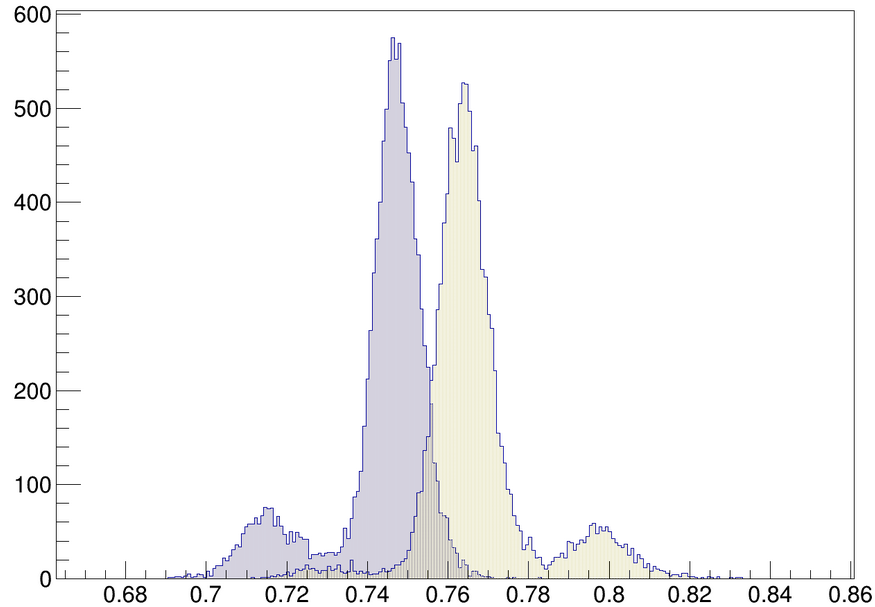
\includegraphics[scale=0.5]{images/dual-mode-gaussian.png}
\end{center}
\caption{\label{dual-mode-gaussian} Distribution of the number of events per 
second (evt/sec) collected from VMs with 8 virtual CPUs. }
\end{wrapfigure}

\section{Distribution of the performance samples}
KV was executed on 240 Haswell-EP hypervisors providing compute
resources as VMs dedicated to the Tier-0 batch system. The servers were
fitted with two 8-core Intel Xeon E5-2630v3 processors, with a total number  
of 32 threads per server with simultaneous multithreading enabled, and 64GiB    
of DDR4 RAM in fully balanced configuration, with each memory channel populated with
the same number of DIMMs of equal capacity. All the hypervisors were configured 
to host 4 VMs providing 8 virtual processing units each, with pairs of VMs 
confined to separate NUMA domains. KV was executed with 8 parallel processes 
on each VM, resulting in the full utilization of the hardware threads provided
by the machine, and the final aggregated result was obtained as the average over 
the 8 simulation times. The samples collected from the VMs under test resulted in a 
dual-mode guassian distribution, with a 2\% difference between the 
mean of the two modes as shown in figure 
~\ref{dual-mode-gaussian}.

\section{Bare metal results}
In order to ease the performance analysis, the virtualization layer was
temporarily removed and Simultaneous Multithreading disabled, running KV on 
the bare-metal server while setting scheduling affinity sequentially to each physical
core. The results shown
in figure ~\ref{kv-runtime} highlighted a 12\% difference in the average simulation
time when binding KV to core 8, the first core of the second processor, i.e. CPU1.

\begin{figure}[b]
\begin{center}
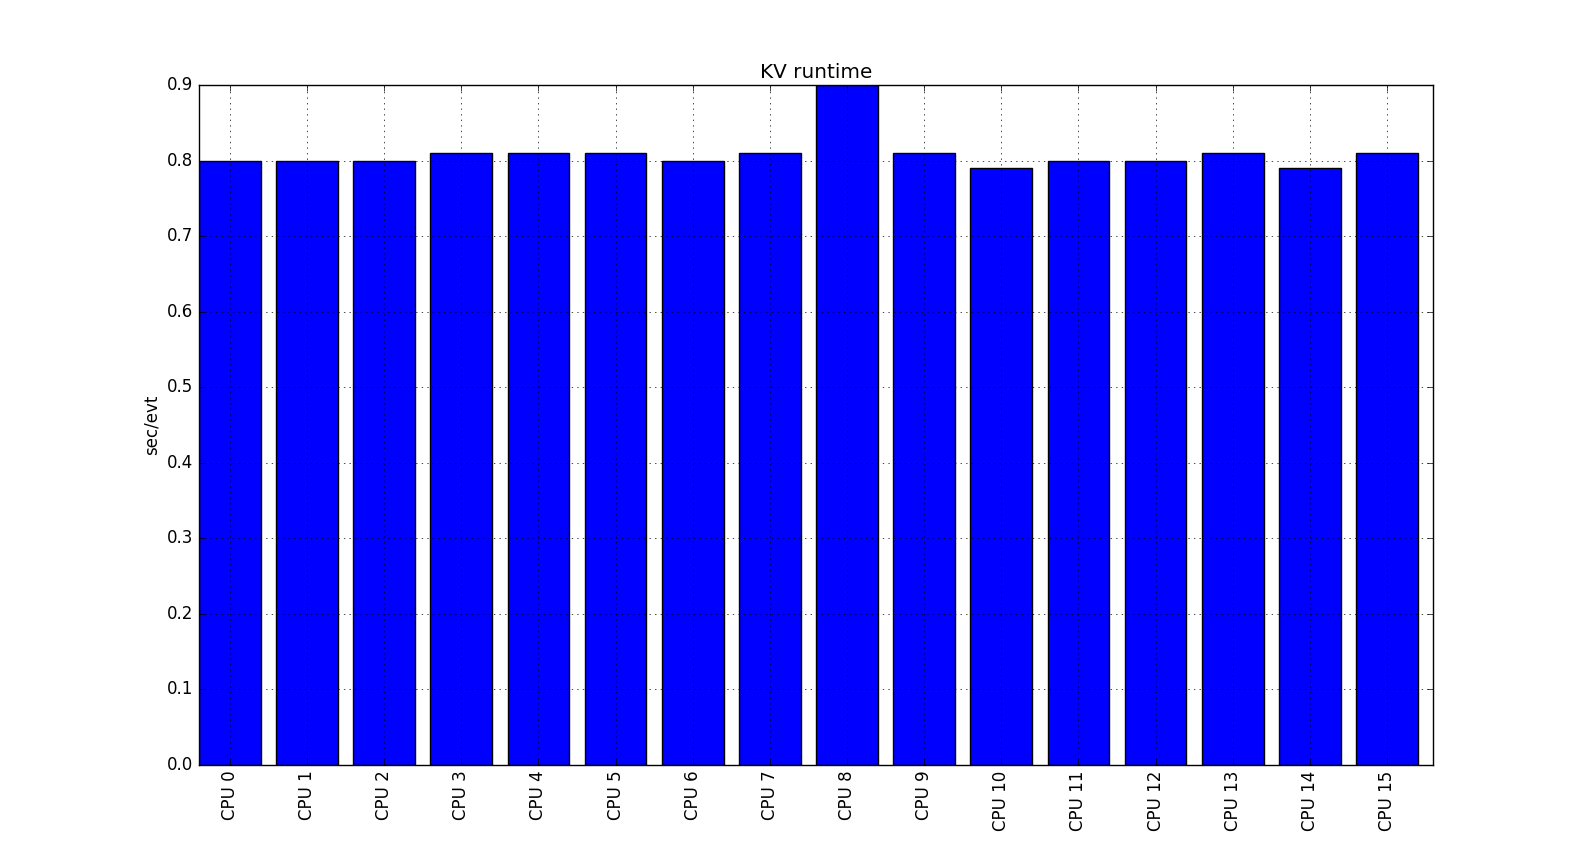
\includegraphics[scale=0.3]{images/kv_runtime.png}
\end{center}
\caption{\label{kv-runtime} Bare-metal KV performance (sec/evt) on each physical core. }
\end{figure}
Further tests confirmed the same behavior also with Simultaneous Multithreading 
on, with slower performance on thread 8 and 24, both belonging to the first core of 
CPU1. Single thread runs in a virtualized environment showed a 16\%
increase in the final average simulation time when running on virtual processors
corresponding to hardware threads 8 and 24, confirming the 2\%
spread that stood out from the statistical distribution after averaging the results
over all 8 virtual processors within each VM. 


\section{Profiling single events}
A deeper dive in the logs showed that all the events required more time to be 
simulated on the first core of CPU1. In particular, event 73 was identified as the one
requiring the longest simulation time: ~34 seconds on core 8 against ~29 seconds
on any other core, making it a good candidate for an in-depth analysis. Profiling 
a single event required a way to attach \textit{perf} to KV only during the time frame
where one specific simulation was being executed. The solution adopted consisted
in a Python script which would monitor KV log files via \textit{pyinotify} to detect
the beginning of event 73. The script would attach \textit{perf} to KV until the
detection of the end of event. One essential requirement for this to work correctly
was to disable all the buffering carried out at any layer of the stack before
data actually reaching the storage device. KV writes log files via Python code,
therefore the following points had be taken into consideration:
%\begin{lstlisting}[caption=Simulation of event 73 on core 8, basicstyle=\scriptsize]
%*  Memory snooper called at end of event with VMEM: 1443232kB
%G4SimTimer           INFO        Event nr. 73 took 34.58 s. New average 0.985 +- 0.4806
%AtRndmGenSvc         INFO  Stream =  SINGLE, Seed1 =  93448506, Seed2 = 144728191
%AthenaEventLoopMgr   INFO  done processing event #72, run #1 73 events processed so far
%AthenaEventLoopMgr   INFO  start processing event #73, run #1 73 events processed so far
%G4AtlasAlg           INFO ++++++++++++  G4AtlasAlg execute  ++++++++++++
%\end{lstlisting}

%\begin{lstlisting}[caption=Simulation of event 73 on core 0, basicstyle=\scriptsize]
%*  Memory snooper called at end of event with VMEM: 1443252kB
%G4SimTimer           INFO        Event nr. 73 took 29.68 s. New average 0.8681 +- 0.4133
%AtRndmGenSvc         INFO  Stream =  SINGLE, Seed1 =  93448506, Seed2 = 144728191
%AthenaEventLoopMgr   INFO  done processing event #72, run #1 73 events processed so far 
%AthenaEventLoopMgr   INFO  start processing event #73, run #1 73 events processed so far
%G4AtlasAlg           INFO ++++++++++++  G4AtlasAlg execute  ++++++++++++
%\end{lstlisting}

\begin{itemize}
\item A call to \textit{open} function in Python, results in the invocation
of libc \textit{fopen}. Python can modify libc buffering behaviour via libc 
function \textit{setvbuf} if \textit{buffering} parameter is specified, 
otherwise the default libc buffering is used. Without control over the Python
source code, its it not possible to modify buffering options.
\item Environment variable \textit{PYTHONUNBUFFERED} can be used to turn off
buffering of \textit{stdin, stdout, stderr}.. 
\end{itemize}
The best solution found to implement unbuffered I/O to log files was to set 
\textit{PYTHONUNBUFFERED=1} and pipe logs printed by KV on standard output to
\textit{tee}, which would eventually write to an additional log file setting 
\textit{\_IONBF} on all file descriptors via \textit{setvbuf}.
\textit{unbuffer} command was also used to disable buffering between the two
ends of the pipe. 
\\
\textit{perf record} was used to profile the execution. Results for core 8 
are shown in figure ~\cite{event-73-processor8}, and results for core 9 are 
shown in figure ~\cite{event-73-processor9}.

\begin{figure}[h]
\begin{center}
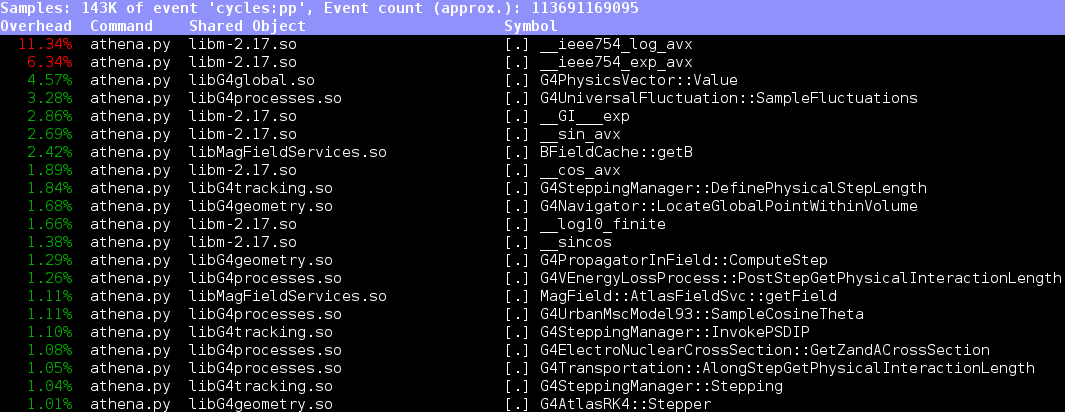
\includegraphics[scale=0.45]{images/Event73_Processor8.png}
\end{center}
\caption{\label{event-73-processor8} Recording of event 73 on core 8}
\end{figure}

\begin{figure}[h]
\begin{center}
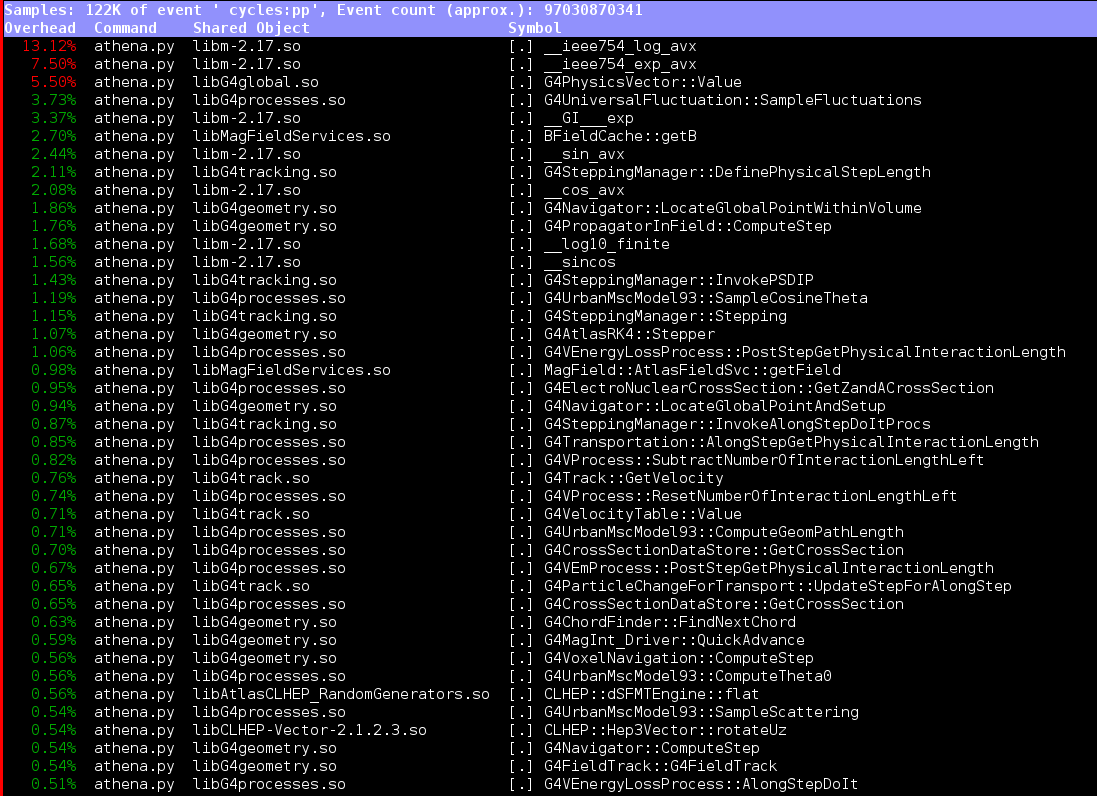
\includegraphics[scale=0.45]{images/Event73_Processor0.png}
\end{center}
\caption{\label{event-73-processor9} Recording of event 73 on core 0}
\end{figure}

\section*{References}
\bibliography{iopart-num}
\bibliographystyle{unsrt}
\end{document}
